\documentclass[lang=cn,11pt,a4paper,cite=authornum]{paper}

\title{Linux开发环境及应用\ 上机作业四:Shell管道和重定向功能的实现\ 实验报告}
\author{毛子恒 \\ 2019211397}
\institute{北京邮电大学\ 计算机学院}

\date{\zhtoday}

\setmonofont{Consolas}

% 本文档命令
\nocite{*}

\begin{document}

\maketitle

\section{实验内容}

使用\mintinline{C}{fork()},\mintinline{C}{exec()},\mintinline{C}{dup2()},\mintinline{C}{pipe()},\mintinline{C}{open()},\mintinline{C}{wait()}等系统调用编写C语言程序完成与下列Shell命令等价的功能。

\mintinline{shell}{grep -v usr < /etc/passwd | wc –l > r.txt; cat r.txt}

\section{实验步骤}

\paragraph{编写代码}

使用\mintinline{C}{pipe()}初始化管道,\mintinline{C}{fork()}创建子进程,\mintinline{C}{open()}打开文件,\mintinline{C}{dup2()}重定向文件描述符,\mintinline{C}{execlp()}执行程序。

\begin{code}
\begin{minted}{C}
#include <fcntl.h>
#include <stdio.h>
#include <unistd.h>
#include <sys/types.h>
#include <sys/stat.h>
#include <sys/wait.h>

int main()
{
    int fd[2];
    pipe(fd);
    if (!fork())
    {
        close(fd[0]);
        int passwd_fd = open("/etc/passwd", O_RDONLY);
        dup2(passwd_fd, 0);
        dup2(fd[1], 1);
        close(fd[1]);
        execlp("grep", "grep", "-v", "usr", NULL);
    }
    if (!fork())
    {
        close(fd[1]);
        int r_fd = open("r.txt", O_WRONLY | O_CREAT, 0777);
        dup2(fd[0], 0);
        close(fd[0]);
        dup2(r_fd, 1);
        execlp("wc", "wc", "-l", NULL);
    }
    wait(NULL);
    close(fd[0]);
    close(fd[1]);
    execlp("cat", "cat", "r.txt", NULL);
}
\end{minted}
\end{code}

\paragraph{运行结果}

运行结果如\figref{fig:p1}。

\begin{figure}[!htb]
    \centering
    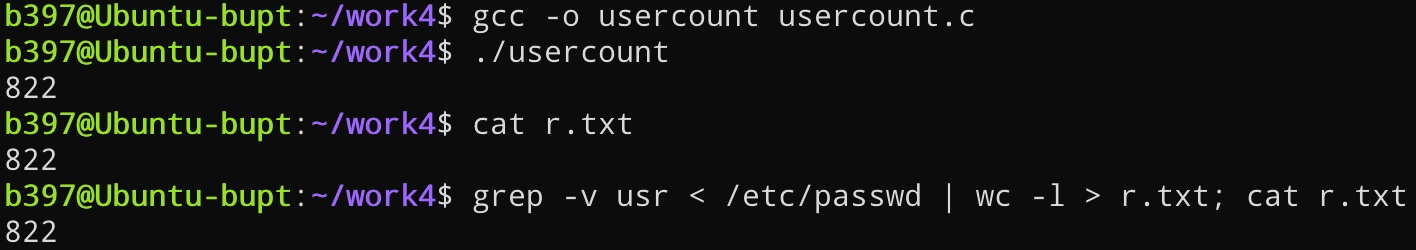
\includegraphics[width=0.8\textwidth]{./images/l4.jpg}
    \caption{运行结果\label{fig:p1}}
\end{figure}

\section{实验总结}

本次实验中我主要应用了\mintinline{C}{fork()},\mintinline{C}{exec()},\mintinline{C}{dup2()},\mintinline{C}{pipe()},\mintinline{C}{open()},\mintinline{C}{wait()}系统调用模拟了shell的一小部分功能,使我对进程管理和文件描述符更加熟悉。

\end{document}